\documentclass{article}

\usepackage{parskip}
\usepackage{amsmath}
\usepackage{amssymb}
\usepackage{esvect}
\usepackage{xfrac}
\usepackage{tikz}
\usetikzlibrary{positioning, angles}

\renewcommand{\contentsname}{Lesson 3}

\begin{document}

\newpage
    \tableofcontents
\newpage

\section{Newton's Laws}

\begin{itemize}
    \item Philosphiae Naturalis
    \item Principia Mathematica in 1687
\end{itemize}

\subsection{Newton's First Law}

An object in motion moves in staight lines at constant speed unless acted upon by an external force

\begin{itemize}
    \item \textbf{Inertia} - ``Reisistance to change" in velocity
    \item \textbf{mass (m)} - Inertia of a physical object
        \begin{itemize}
            \item More mass = More resisitance to change
        \end{itemize}
\end{itemize}

\subsection{Newton's Second Law}

A force is the change in momentum (p) per unit time

\textbf{force (F)} – first derivative of \textit{momentum} WRT \textit{time}

\textit{* WRT – With respect to}

$$ \sum \vv{F}_{ext} = \frac{ d\vv{p} }{dt} $$

$$ g(x,t) $$
$$ g' = \frac{dg}{dx} $$
$$ \dot{g} = \frac{dg}{dt} $$

$$ \vv{p} = m\vv{v} $$
\begin{align*}
    \sum \vv{F}_{ext} & = \vv{\dot{p}} \\
                      & = m\vv{dot{v}} + \dot{m}\vv{v}
\end{align*}
\begin{equation*}
    \boxed{\sum \vv{F}_{ext} = m\frac{d\vv{v}}{dt}}
\end{equation*}

There are only a handful of forces. There are two broad categories:

\begin{equation*}
    \begin{tabular}{ c | c }
        Long Range & Contact \\
        \hline
        Gravity (1A) & Friction \\
        Electromagnetic (1C) & Normal \\
        Strong (1D) & Applied \\
        Weak (1D) & Tension \\
                  & Orange \\
                  & Drag (1B)
    \end{tabular}
\end{equation*}

\textit{* Text within parenthesis refers to physics courses where the force is covered in detail}

Force definitions
\begin{itemize}
    \item \textbf{Normal force (N)} - Perpendicular to surface of contact, and always points away from the surface
    \item \textbf{friction (f)} - Parallel to contact surface
        \begin{itemize}
            \item $ f = \mu N $
            \item $ \mu $ – ``coefficient of friction"
        \end{itemize}
    \item \textbf{Tension ($ F_{T},T $)} - Carried along a rope or change \& points away from the object
        \begin{itemize}
            \item Tension is \underline{not} uniform if: rope has mass, massive pulley
        \end{itemize}
\end{itemize}

\subsection{Newton's Third Law}

Every force creates a reaction force which acts on a different object. These forces are equal in magnitude and opposite in direction.

Drawing a diagram
\begin{enumerate}
    \item Draw a simplified diagram
    \item Identify points of contact
    \item List all relevant forces
    \item Draw a free body diagram
\end{enumerate}

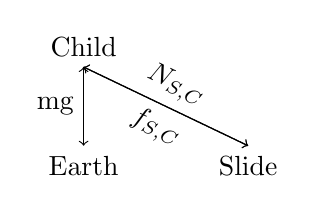
\begin{tikzpicture}
    \draw[rectangle, very thick] node (child) {Child};
    \draw[rectangle, very thick] node (earth) [below=of child] {Earth};
    \draw[rectangle, very thick] node (slide) [right=of earth] {Slide};

    \draw[<->] (child.south) -- (earth.north) node[midway, left] {mg};
    \draw[<->] (child.south) -- (slide.north) node[midway, above, sloped] {$ N_{S,C} $};
    \draw[<->] (child.south) -- (slide.north) node[midway, below, sloped] {$ f_{S,C} $};
\end{tikzpicture}

\textbf{Static} -
$$ \frac{d\vv{v}}{dt} = 0 $$
$$ \sum F_{ext} = 0 \text{, if $ m $ = 0} $$

What value does $ \mu $ have if $ m $, $ g $, \& $ \theta $ are known?

\begin{tikzpicture}
    \draw[->] (0,0) -- (135:3cm) node [above] {$ f $};
    \draw[->] (0,0) -- (45:3cm) node [above] {$ N $};
    \draw[->] (0,0) -- (-90:3cm) node [below] (gravity) {$ mg $};
    \draw[dashed, ->] (0,0) -- (-135:3cm) node [midway, above, sloped] (mgy) {$ mg_y = mg\cos(\theta) $};
    \filldraw[black] (0,0) circle(2pt);
\end{tikzpicture}

$$ f = \mu N $$
Always start with a $ \sum F $ statement

$ x $ Direction:
$$ \sum F_x^{(m)} = 0 $$
* Where $ x $ is direction and $ (m) $ is the object
$$ mg\sin(\theta) - f = 0 $$
$$ f = mgsin(\theta) $$

$ y $ Direction:
$$ \sum F_y^{(m)} = 0 $$
$$ N - mg\cos(\theta) = 0 $$

$$ f = \mu N $$
$$ mg\sin(\theta) = \mu(mg\cos(\theta)) $$
$$ \mu = \frac{\sin(\theta)}{\cos(\theta)} = \tan(\theta) $$

\section{Density}

\textbf{Density}:
$$ \frac{dm}{dy} = \frac{M}{L} $$
$$ dm = \frac{M}{L}dy $$
$$ dT = gdm $$
$$ \int_0^T dT = \int_0^y \frac{Mg}{L} dy $$
$$ T = \frac{Mg}{L}y $$

\end{document}
